\documentclass[11pt]{amsart}

\usepackage[utf8]{inputenc}
\usepackage{amsmath}
\usepackage{physics}
\usepackage{graphicx}

\renewcommand{\thesubsection}{\thesection.\alph{subsection}}

\title[Problem Set 4]{Semiconductors and Metals\\
			\hrulefill \small{ FYS3410: Problem Set 4 } \hrulefill}

\author{Candidate 33}

\date{\today}

\begin{document}

\maketitle

\setcounter{section}{2}

\section{Gallium Arsenide Semiconductor}
Gallium arsenide (GaAs) is a semiconductor with a direct band gap of $~1.42eV$ at room temperature. The experimental values for effective masses (in unit of free electron mass) are: $0.067$, $0.082$ and $0.45$ for electrons in the conduction band as well as light and heavy holes at the of the valence bands, respectively. 

The band structure of some semiconductors, including GaAs, around the point $\Gamma$ can be approximated by
\begin{equation}
E(\vb{k}) = E_0 + \frac{\hbar^2}{2m^*}(\vb{k}^2 - \Gamma) = C + Ak^2,
\end{equation}
where $m^*$ is the effective mass, and the factor $A$ is the curvature of the band. Setting $C=E_0=0$ one gets
\begin{equation}
A = \frac{\hbar^2}{2m^*}.
\end{equation}
Inserting for the different effective masser of the electrons and holes yields
\begin{align*}
A_1(m^* = \ \  0.067m_0) &= \ \ 0.569eVnm^2 \\ 
A_2(m^* = -0.082m_0) &= -0.465eVnm^2 \\
A_3(m^* = -0.450m_0) &= -0.085eVnm^2.
\end{align*}

\begin{figure}
\centering
	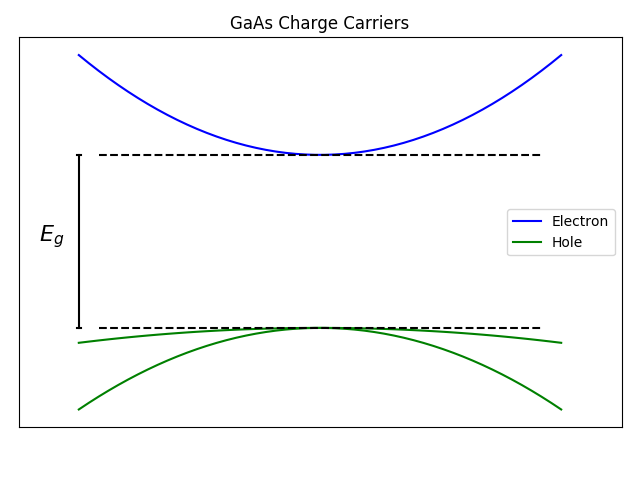
\includegraphics[width=0.75\textwidth]{problem3.png}
	\caption{Band gap in the vicinity of $\Gamma$ point. The effective mass of the holes (valence band) and electrons (conduction band) can be determined from the curvature of the graphs.}
	\label{fig:problem3}
\end{figure}

Figure \ref{fig:problem3} shows the band gap in the vicinity of $\Gamma$. The curvature of the energy level in $k$-space gives an indication to how heavy the hole or electron is. A steep curve gives light holes/electrons and a more moderate curvature means that the hole/electron is heavy.

\section{Hydrogen-like Dopants}


\end{document}